\chapter{Survey}
\label{chapter:Survey}

In this chapter, to answer the question ``Do projections of Drools business rules lead to greater understanding of those rules?'', we undertook a survey research.
In section \ref{section:section:survey_method} we describe the method of this survey.
Section \ref{section:section:survey_results} examines the outcomes of our research.
Finally, in section \ref{section:section:survey_discussion} we discuss the threats to validity of our approach.

\section{Method}
\label{section:survey_method}

We tested the validity of the prototype using a survey.
If a survey is not well designed, then it could lead to invalid or irrelevant outcomes.
This chapter describes the design and procedure of the survey.
Additionally, it outlines any threats to its validity.
Our choice of survey technique is a questionnaire.

\subsection{Questionnaire Design}
To design the survey of our prototype, we followed the following rules derived from the works of Bryman\cite{bryman2016social} and de Vaus\cite{de2013surveys}.

\begin{itemize}    
    \setlength\itemsep{0em}
    \item \emph{Introduction:} 
        We devised a clear introduction to describe the research.
    \item \emph{Existing work:} 
        We considered existing questions.
        Regarding projectional editing, we requested the original questionnaires from three papers\cite{meacham2020adaptivevle_SLR,berger2016efficiency, voelter2014towards} about tools developed using projectional editing.
        Unfortunately, none of the original questions were available for assessment.
    \item \emph{Question in mind:} 
        We had the specific research question, ``Which projections can help developers get appropriate feedback about rules?'' in mind when formulating the questions.
    \item \emph{Succinct:} 
        The pool of Drools users that we were personally in contact with was tiny.
        Thus, we had to rely on responses from strangers.
        For this reason, we tried to make the questionnaire as quick to finish as possible.
        This constraint meant we looked particularly hard at removing questions that did not help us to our research goal.
    \item \emph{Pilot:} 
        We piloted the questionnaire with both ourselves and our industrial supervisor. 
        The result of this pilot led to more explanative text before the questions.
    \item \emph{Clarity:} 
        The instructions to each of the questions were tested for clarity by a non-technical third party.
        We took care to rework questions that were long, ambiguous, general, or leading not to be so.
        We also took care to remove jargon, negative wording, and questions that asked about more than one thing.
    \item \emph{Closed questions:} 
        The only open questions were ones from which we wished to extract sentiment.
        To avoid binary questions, where appropriate, we applied a Likert scale\cite{likert1932technique}.
    \item \emph{Single page questions:} 
        Thanks to the UI of Survey Monkey, no questions spanned multiple pages.
    \item \emph{Important questions first:} 
        We started with the research-based questions, leaving the socio-demographic questions, such as skill level, to the end.
\end{itemize}

Appendix \ref{Appendix:Questionaire_text} shows the questionnaire we designed following these principles.


\subsection{Participants}

The requirement for participants is that they have at least a little experience with using Drools.
We hoped to get a statistically significant number of participants.

\subsection{Validity}
We addressed the non-response bias\cite{armstrong1977estimating} by making the questionnaire short and easy to answer.
Because of the nature of the participant selection for this survey, it will be challenging to address the self-selection bias caused by the voluntary nature of the response.

Common method bias, i.e., ``variance that is attributable to the measurement method rather than to the construct the measures represent''\cite{podsakoff2003common} can be responsible for 25\% or more of variable relational influence.
As we are only conducting a single survey, we will not be able to prevent this. 
However, we took the following small precautions.
We tested the survey to remove question ambiguity, mood influences, and length issues.
We mixed the order of questions in the survey to mitigate the issues caused by the similarity, proximity, and location of items.
We varied the scales and order of our Likert scales.

The main statistical methods to address common method bias, i.e., ``Harman's single factor test''\cite{podsakoff2003common} and the ``marker variable''\cite{lindell2001accounting} have been found to be lacking in grounding\cite{gorrell2011countering}.
The marker variable approach is appropriate if used with caution.
However, it may not be possible to gain a statistically significant outcome with our expected response size.

\subsection{Pre-test}
We sent our first pass of the survey to our industrial supervisor, who has experience with Drools.
With this pre-test, we hoped to remove ambiguously worded or leading questions.
Additionally, we wanted to confirm that the questionnaire took around 10 minutes to complete.

As a result of this pre-test, we updated much of the explanatory text.

\subsection{Sampling}
Within our professional network, we only had a connection with very few Drools developers.
We also considered that having acquaintances answer the questionnaire could introduce some biases we could not account for.
So, we had to expand our sampling reach.

Our first approach was to search StackOverflow for question askers and answerers about Drools.
Our preference was to find email addresses, failing that Twitter contacts.
Unfortunately, this proved quite limited.
We only managed to harvest 13 email addresses, and six Twitter handles.

Our following approach was to interrogate our LinkedIn connections for anyone who claimed Drools as one of their marketable skills.
At two degrees of separation in our LinkedIn network, we found 204 candidates with Drools skills listed.
From these, we harvested 54 email addresses, and 40 Twitter handles.

We chose not to expand our search to three degrees of separation.
At two degrees of separation, we share a relationship with the same person.
We thought it would be harder to take advantage of the social pressure to answer when we do not have that shared relationship.

\subsection{Procedure}

The questions, as described in appendix \ref{Appendix:Questionaire_text}, were turned into a survey using the Survey Monkey service.
We also show screenshots of one version of the questionnaire in appendix \ref{Appendix:Questionaire_text}.

To encourage response, we crafted a short introduction email, heavily relying on techniques designed to enhance response as discussed by  Cialdini\cite{goldstein2008yes}.

\newpage
\section{Results: Survey}
\label{section:survey_results}

\subsection{Population Selection}
We initially had two sources to find experienced Drools users to be subjects of our survey.
From LinkedIn, we selected users who were at two degrees of separation from us and listed Drools in their skills.
From StackOverflow, we selected users who had asked or answered questions about Drools. 

In these two websites, the users do not typically list their contact details.
Some investigation was required.
From the initial selection, we harvested email addresses and, failing that, Twitter handles.

Following this, we determined that academic papers could be a good source of a population of expertise.
We used Google Scholar to look up Drools papers from the previous two years.
After skimming the papers to ensure that they were explicitly about or using the Drools language, we harvested email addresses from them.

On the second and fourth day after the initial sending of the survey, two subjects forwarded a web link to mailing lists.
A developer from the core Drools team sent it to a list of known Drools consultants.
The other sent it internally in his company.
The subjects who sent the survey to their mailing list forwarded links to version C of the survey.

We had created four versions of the questionnaires to combat the single source bias.
We distributed the surveys to the subjects harvested from LinkedIn and StackOverflow evenly.
There was an overrepresentation of Survey C because of the mailing lists.
Therefore, we distributed the subjects harvested from academic papers evenly over Surveys A, B and D.

We show the collection results in figure \ref{fig:Survey_participants}.
We see here that the collection method did not have much of an impact on return rates.
Whilst StackOverflow had a higher rate, the number of people contacted was small, thus having an outsized effect on the response rate.

The first three pie charts represent the collection methods over which we had control.
These three represented 24 of our 30 completed questionnaires.
The last pie chart represents six completed and four partially completed questionnaires returned from the mailing lists.
We do not know the size of the starting population of these mailing lists. 
Thus, this pie chart only shows the ratio of partial to completed results.

In summary, a survey reached 154 potential participants, of which 24 completed it, for a Response Rate of 15.5\%.
In addition, an unknown number of potential participants were reached through mailing lists, returning a further six completed surveys.

\subsection{Participant Demography}

Responses came from around the world.
Figure \ref{fig:Survey_locations} shows that most respondents reside in Europe, except for one in each of the USA, Israel, and Singapore. 
Italy and the Netherlands provided the most significant number of responses, with 7 and 5 respectively.

The experience of our subjects was relatively high.
As can be seen in \ref{fig:sfig1}, most of our subjects have over ten years of programming experience.
17\% of our recipients had a low experience of Drools, and 30\% were very experienced, as shown in figure \ref{fig:sfig2}.
Figure \ref{fig:sfig3} shows that 40\% of our recipients had used Drools in this current year, and 30\% had not used it in the last five years.

\begin{figure}
    \centering
    \fbox{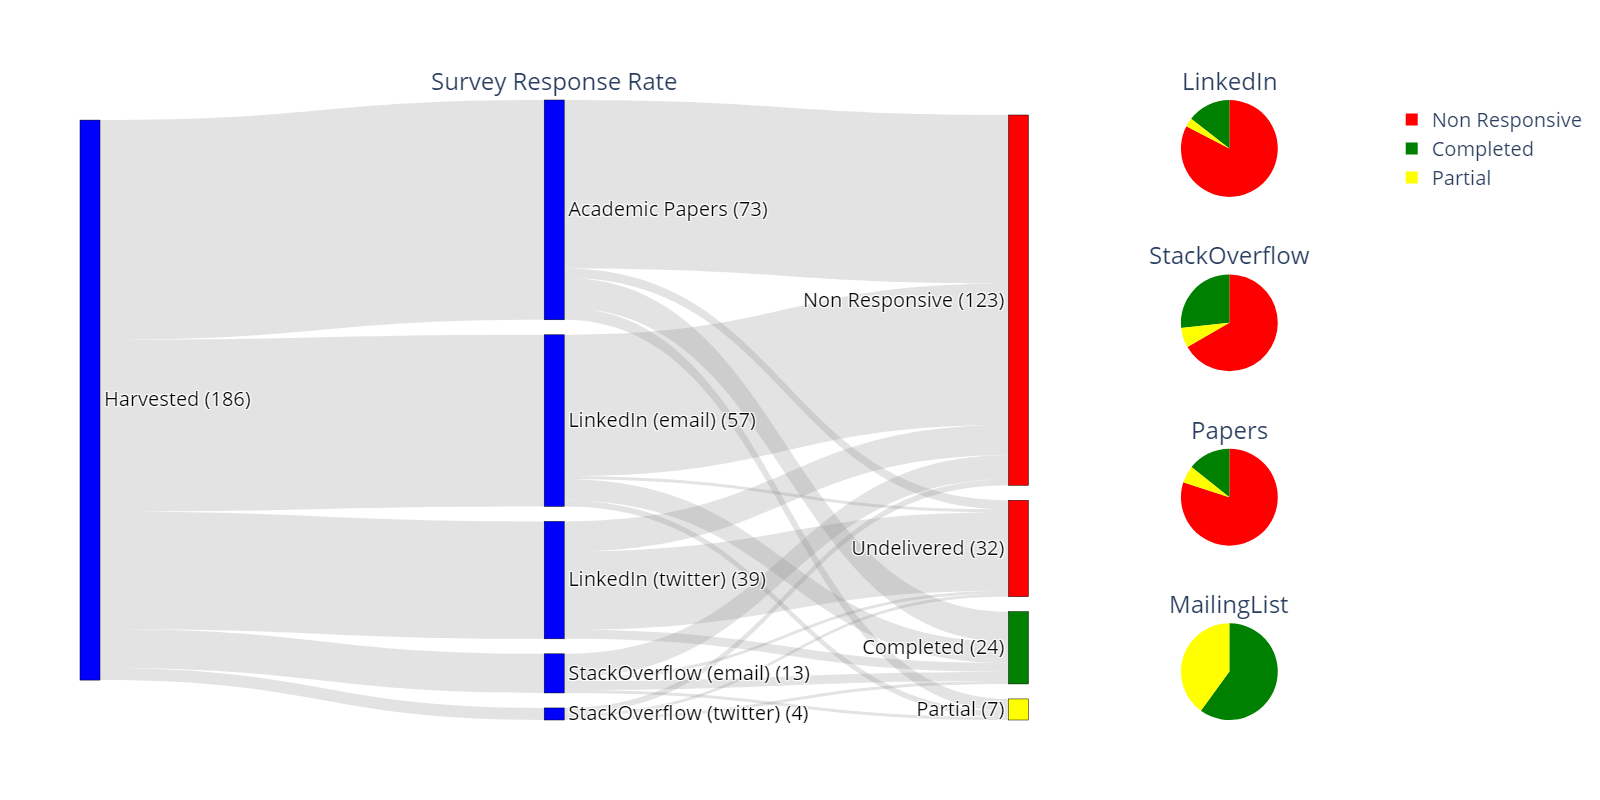
\includegraphics[width=0.95\textwidth]{Sections/images/survey_participants-2.png}}
    \caption{Survey participants}
    \label{fig:Survey_participants}
    \fbox{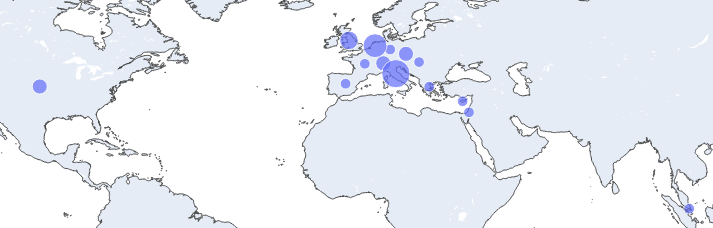
\includegraphics[width=0.95\textwidth]{Sections/images/survey_locations.png}}
    \caption{Survey locations}
    \label{fig:Survey_locations}
    \begin{subfigure}{.33\textwidth}
      \centering
      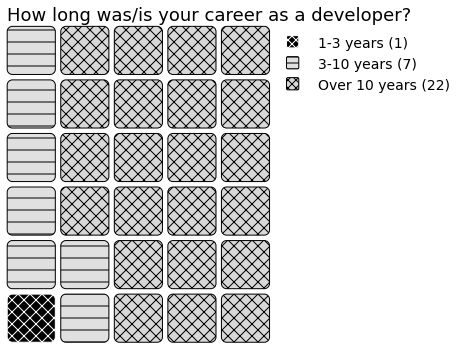
\includegraphics[width=.95\linewidth]{Sections/images/pie_experiencer4.png}
      \caption{SE experience}
      \label{fig:sfig1}
    \end{subfigure}%
    \begin{subfigure}{.33\textwidth}
      \centering
      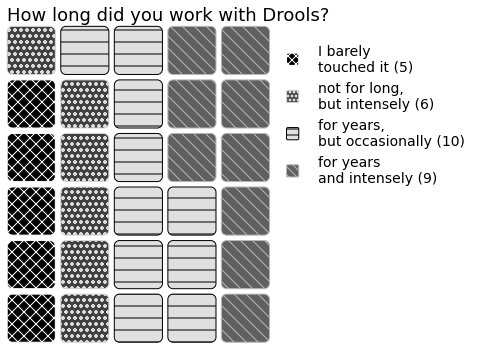
\includegraphics[width=.95\linewidth]{Sections/images/pie_droolsExperience4.png}
      \caption{Drools experience}
      \label{fig:sfig2}
    \end{subfigure}
    \begin{subfigure}{.33\textwidth}
        \centering
        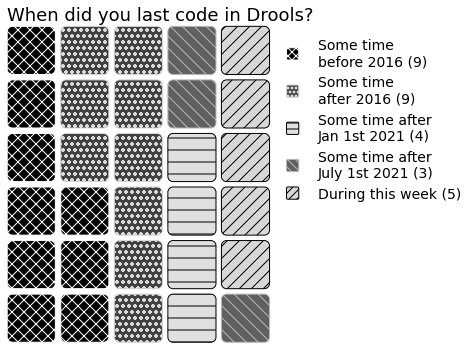
\includegraphics[width=.95\linewidth]{Sections/images/pie_recentusage4.png}
        \caption{Recent use}
        \label{fig:sfig3}
      \end{subfigure}
    \caption{Subject experience}
    \label{fig:subject_experience}
\end{figure}

Half of our subjects reported only ever using one editor for Drools, with the slight majority of those only using Eclipse.
Eclipse also had the most instances of reporting of having been used.
Out of the 55 instances of editors reported as being used, 20 of those were Eclipse.
There was a surprising diversity of tools used.
The purpose of this section was to calibrate responses against exposure to IDEs with greater Drools Support.
The wide diversity of editor usage and high incidence of multiple editor usage means that these answers are not suitable for use in the sub-categorisation of responses. 
We show the distribution of usage in figure \ref{fig:editorUsage} on page \pageref{fig:editorUsage}.

\begin{figure}[h]
    \centering
    \fbox{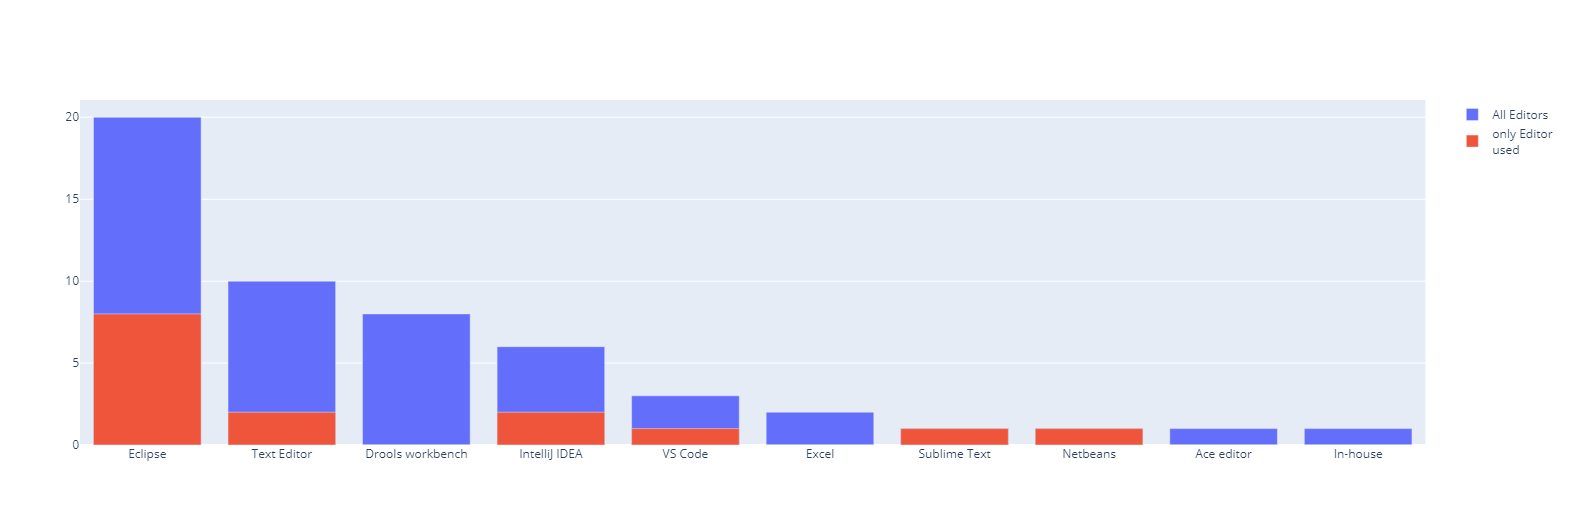
\includegraphics[width=0.95\textwidth]{Sections/images/EditorUseage.png}}
    \caption{Editors used}
    \label{fig:editorUsage}
\end{figure}

\subsection{Question Analysis}

\subsubsection{Grouping}
When displaying subtypes, we shall split them into groups.
The source of the response will create a pseudo-cross-section of our participants.
The ten contacted through academic papers will be considered our academics.
The remaining 20 will be considered practitioners.

The next grouping is based on Drools Experience.
The nine who replied they had used Drools ``for years and intensely'' are categorised as experts.
The 16 who either answered ``for years, but occasionally'' or ``not for long, but intensely'' we categorise as seniors.
The five who answered ``I barely touched it'' are categorised as novices.

Another grouping will be on recency of use.
The 12 who have used Drools in 2021 are categorised as current users, the remaining 18 as past users.

To remove some bias in the questionnaires, we changed question order, order of projections and used rule sets.
When a question is affected by this, then this segregation will also be displayed.

\subsubsection{Display}
For the remainder of this results section, whilst displaying results that regard our Likert scaled questions, we will be following the advice of Robbins et al.\cite{robbins2011plotting} by using diverging stacked bar charts, with counts added.
This style allows the evaluation of the results of subclasses.
The addition of counts makes it easier to spot when small numbers skew the results.

In our charts, we will place positive scores to the right of the centre line and neutral and negative scores to the left.
Our particular question design cannot tell if the neutral responses are substantive or hidden non-responses\cite{blasius2001use}.

\subsubsection{Grouping Analysis}
Our data does not fall under a normal distribution. 
So, we will be using nonparametric analysis.
Vaus\cite{de2013surveys} advises that when analysing ordinal variables with nominal grouping variables, then the statistical methods one should use for checking for differences between groupings would be the Mann-Whitney\cite{mann1947test} or the Kruskal Wallis\cite{kruskal1952use} tests.
In the grouping section, we had one group of only 5 participants, the novices.
As this group is too small to think of using in analysis, we will ignore it.
Ignoring this group means that all the groupings we have are divided into two.
As Mann-Whitney is a specialisation of Kruskal Wallis for two groups, this is the analysis we will use.

For all our analyses, our null hypothesis, H\textsubscript{0}, is that there is no difference between the ranks of the two groups. 
Our alternative hypothesis, H\textsubscript{1}, is that there is a difference between the ranks of the two groups.
Our alpha, or significance, level will be 0.05 for no other reason than it seems to be a mutually agreed-upon value within the statistical community and justifying a different significance would take more time than is warranted for the value these analyses will give.
Our sample size is greater than 20. 
Therefore, we can use a Z distribution.

To work out our Z score, we have an alpha level of 0.05 and a two-tailed test.
Thus, we could work the distribution out by using the following formula:
\[U_{1}=n_{1}n_{2}+\frac{n_{1}(n_{1}+1)}{2}-R_{1}\]
However, it is easier to look up in a Z table.
Thus, we have an ``area in body'' of 0.9750, which correlates in the Z Table to a z value of 1.96.
Ergo, our decision rule is, if our z is less than -1.96, or greater than 1.96, we reject our null hypothesis.
\footnote{We carried out the calculations using the Mann-Whitney U Test calculator at \url{https://www.socscistatistics.com/tests/mannwhitney/default2.aspx}}

\subsubsection{Question 1, 2 and 3: First Impressions}

\noindent\begin{minipage}{\linewidth}
    \centering
    \fbox{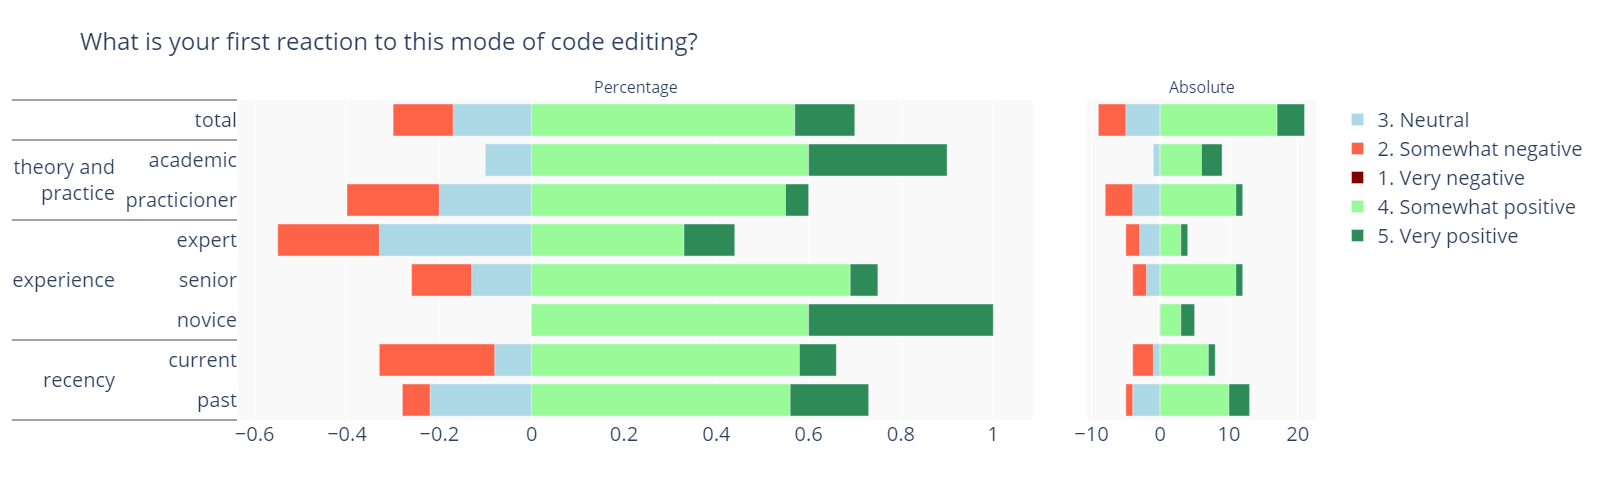
\includegraphics[width=0.95\textwidth]{Sections/images/stackedbar_Q1_2.png}}
    \captionof{figure}{Question 1 - first impressions}
    \label{fig:stackedbar_Q1}
    
    \begin{tabular}{ |l ||r |r |r | r|l | } 
        \hline
        Group Comparison                 & Critical U & U-value & z-Score  & p-value & Hypothesis         \\
        \hline
        \hline
        Academic vs Practitioner         & 55         & 54.5    & -1.97974 & 0.0477  & \textbf{H\textsubscript{1}}  \\ 
        \hline
        Expert vs Senior                 & 37         & 55      & 0.93413  & 0.35238 & H\textsubscript{0} \\ 
        \hline
        Current vs Past                  & 61         & 91      & 0.6985   & 0.48392 & H\textsubscript{0} \\ 
        \hline
    \end{tabular}
    \captionof{table}{Mann-Whitney test question 1 - first impressions}
    \label{table:mannwhitneyQ1}
\end{minipage} 

This question shows the subject an example of projectional editing a Drools file alongside a table projection, as an animated GIF, along with an explanation.
Then she is asked her first reaction. 
The chart in figure \ref{fig:stackedbar_Q1} shows the outcomes.
Eyeballing the chart, we observe that the novice and the academics, where there is much crossover, found the initial presentation more positive than the experienced practitioners.

Table \ref{table:mannwhitneyQ1} shows a significant difference between the academics and the practitioners' first reaction to seeing the projectional editing example.
Here, the academics have a far more positive view of the example than the practitioners.

In general, we see an overwhelmingly positive response.
There were five times as many positive (21) than negative (4) responses.
SurveyMonkey directed those who had a positive or negative response to answer the open questions ``Q2. How would this coding style be useful to your interactions with Drools?'' and ``Q3. What do you find negative with this style of coding?'' respectively.
Figure \ref{fig:wordclouds} shows a visualisation of the subject's responses.

\begin{figure}[h]
    \begin{subfigure}{.60\textwidth}
      \centering
      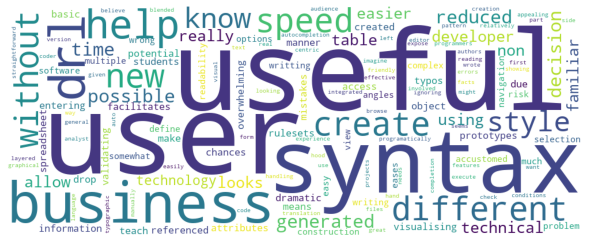
\includegraphics[width=.95\linewidth]{Sections/images/positive_wordcloud.png}
      \caption{Positive}
      \label{fig:wfig1}
    \end{subfigure}%
    \begin{subfigure}{.40\textwidth}
      \centering
      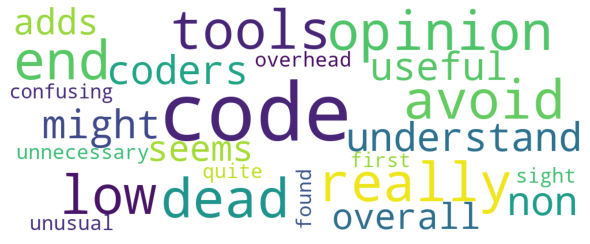
\includegraphics[width=.95\linewidth]{Sections/images/negative_wordcloud.png}
      \caption{Negative}
      \label{fig:wfig2}
    \end{subfigure}
    \caption{Initial thoughts}
    \label{fig:wordclouds}
\end{figure}

Amongst the positive comments, it appears the subjects had picked up on many of the advantages that projectional editing brings.
The ones that got the most mentions, using other words, were exploratory coding, correctness by construction, and multiple viewpoints.
Subjects also noted that, with the projections shown, development could be quicker and easier to check.

Among the few negative comments, they discussed the failures of no/low code solutions, confusing views, and unnecessary overhead.

\subsubsection{Question 4 and 5: Interpret Projection}


\noindent\begin{minipage}{\linewidth}
    \centering
    \fbox{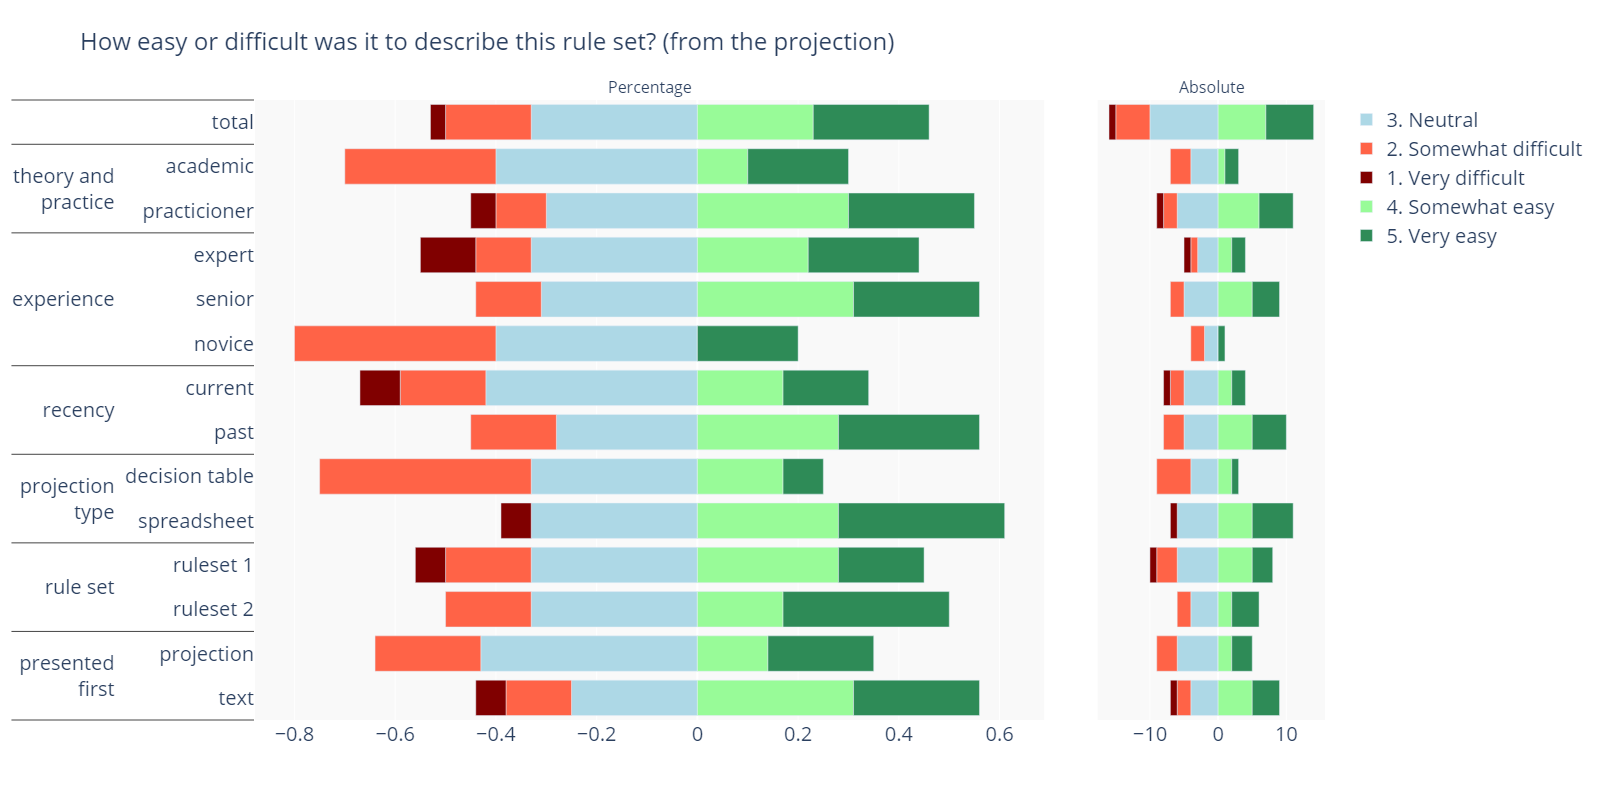
\includegraphics[width=0.95\textwidth]{Sections/images/stackedbar_Q2_2.png}}
    \captionof{figure}{Question 5 - interpret projection}
    \label{fig:stackedbar_Q2}
    
    \begin{tabular}{ |l ||r |r |r | r|l | } 
        \hline
        Group Comparison                 & Critical U & U-value & z-Score  & p-value & Hypothesis         \\
        \hline
        \hline
        Academic vs Practitioner         & 55        & 77      &  0.98987  & 0.32218 & H\textsubscript{0} \\ 
        \hline
        Expert vs Senior                 & 37        & 61.5    &  0.56614  & 0.56868 & H\textsubscript{0} \\ 
        \hline
        Current vs Past                  & 61        & 82.5    &  1.05833  & 0.28914 & H\textsubscript{0} \\ 
        \hline
        Decision Table vs Spreadsheet    & 55        & 61      &  2.2225   & 0.02642 & \textbf{H\textsubscript{1}}  \\ 
        \hline
        Ruleset 1 vs Ruleset 2           & 61        & 92      &  0.65617  & 0.50926 & H\textsubscript{0} \\ 
        \hline
        Projection first vs Text first   & 64        & 97      &  0.60277  & 0.5485  & H\textsubscript{0} \\ 
        \hline
    \end{tabular}
    \captionof{table}{Mann-Whitney test question 5 - interpret projection}
    \label{table:mannwhitneyQ2}
\end{minipage} 

This question asks the subject to describe the meaning of the projection and then describe how hard it was to do that.
Few people described the meaning of the projection well.

The chart in figure \ref{fig:stackedbar_Q2} shows the outcomes.
Looking at the chart, it appears evident that there is a difference in the subjects' confidence between the projections presented.
The participants believed they understood the spreadsheet-style projection better than the decision table projection.

The Mann-Whitney analysis, shown in table \ref{table:mannwhitneyQ2}, confirms this observation.
Otherwise, no other grouping differed significantly from the general population.

The ratio of those evaluating it as easy to those thinking it was hard to understand the projection was ~2:1, 14 to 6.

\subsubsection{Question 6 and 7: Interpret Text}
\noindent\begin{minipage}{\linewidth}
    \centering
    \fbox{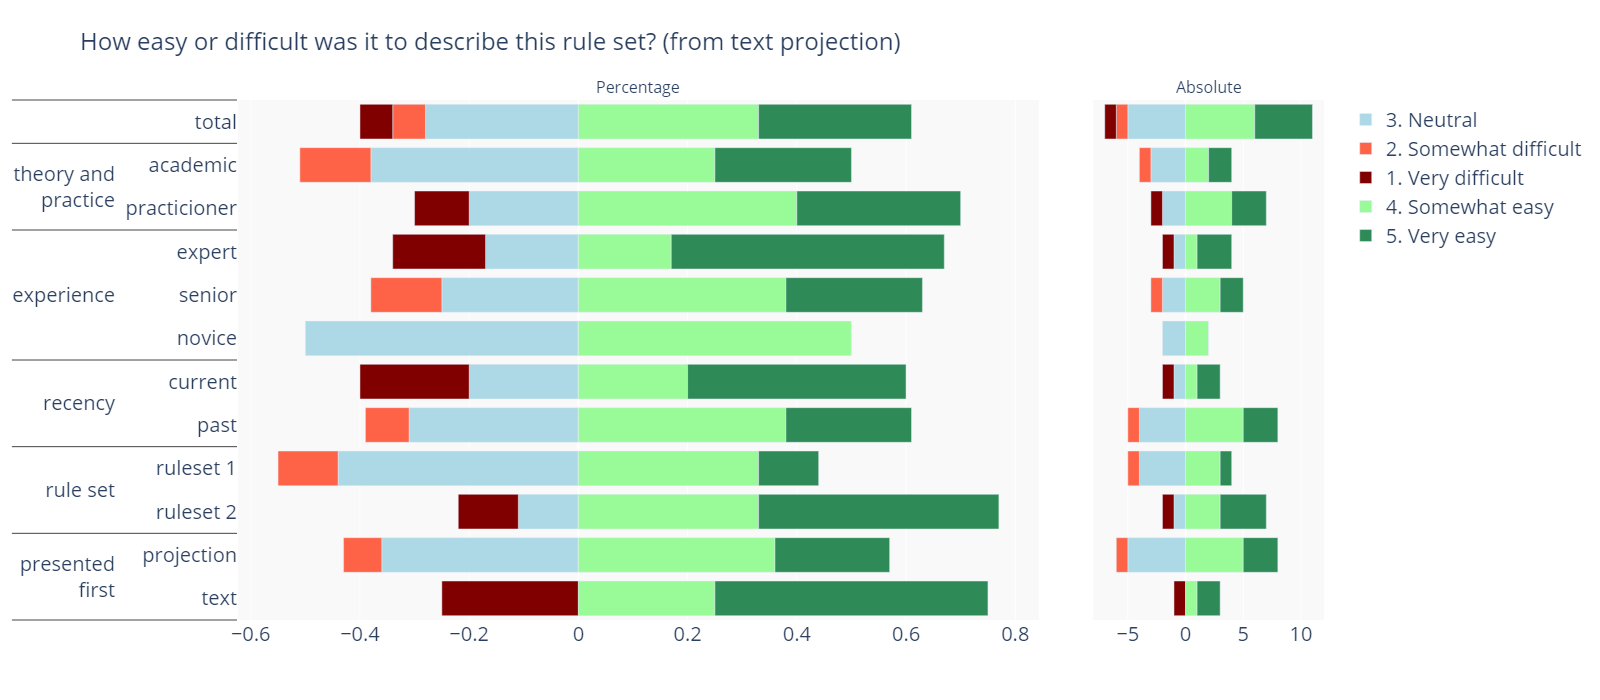
\includegraphics[width=0.95\textwidth]{Sections/images/stackedbar_Q3_2.png}}
    \captionof{figure}{Question 7 - interpret text}
    \label{fig:stackedbar_Q3}
    
    \begin{tabular}{ |l ||r |r |r | r|l | } 
        \hline
        Group Comparison                 & Critical U & U-value & z-Score  & p-value & Hypothesis         \\
        \hline
        \hline
        Academic vs Practitioner         & 17         & 34      &  0.48869 & 0.62414 & H\textsubscript{0} \\ 
        \hline
        Expert vs Senior                 & 8          & 20.5    &  -0.3873 & 0.69654 & H\textsubscript{0} \\ 
        \hline
        Current vs Past                  & 12         & 31.5    &  -0.04929& 0.96012 & H\textsubscript{0} \\ 
        \hline
        Ruleset 1 vs Ruleset 2           & 17         & 24.5    &  -1.36868& 0.17068 & H\textsubscript{0} \\ 
        \hline
    \end{tabular}
    \captionof{table}{Mann-Whitney test question 7 - interpret text}
    \label{table:mannwhitneyQ3}
\end{minipage} 


This question asks the subject to interpret a rule set presented in a Drools style text projection.
The purpose of this question was threefold.
First, to calibrate how well the subject understood Drools.
Second, for comparison with a later projection.
Finally, to calibrate whether and how much easier the text was than the tabular projection to those used to seeing the text version.

Unfortunately, we assume that due to the questionnaire design, there were many non-respondents to this question. 
12 of the 30 respondents did not answer this question.
All 12 of these were from the 16 that were presented the text projection before the tabular projections.

Reporting on 18 responses has significantly less validity.
With that in mind in figure \ref{fig:stackedbar_Q3}, we can see much higher confidence in the easiness of understanding the ruleset.
We see a 5:1 ratio of a greater belief that it was easy to understand the text projections' meaning.
This proportion is significantly higher than those who thought it was easy to understand the tabular projections.

The Mann-Whitney table does not show any significant differences in any of the groups.
We cannot report the difference between those presented with the text projection first or the tabular projection first.
The 4 participants responding from the group presented text first were too low to give a meaningful score.

\subsubsection{Question 8: Compare Projections}
\noindent\begin{minipage}{\linewidth}
    \centering
    \fbox{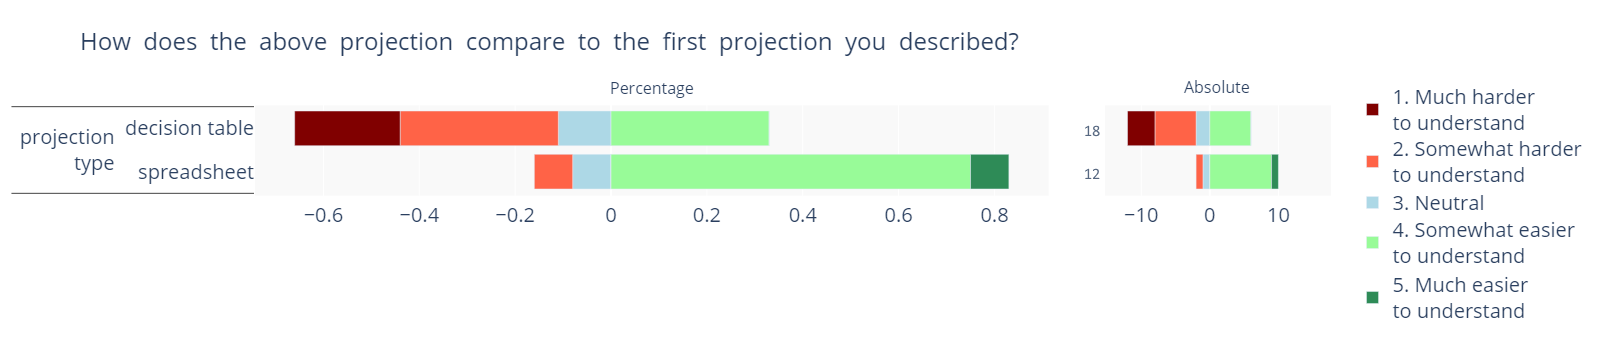
\includegraphics[width=0.95\textwidth]{Sections/images/stackedbar_Q4_2a.png}}
    \captionof{figure}{Question 8 - compare projections}
    \label{fig:stackedbar_Q4}
    
    \begin{tabular}{ |l ||r |r |r | r|l | } 
        \hline
        Group Comparison                 & Critical U & U-value & z-Score  & p-value & Hypothesis         \\
        \hline
        \hline
        Decision Table vs Spreadsheet    & 61         & 45      &  -2.64584& 0.00804 & \textbf{H\textsubscript{1}} \\ 
        \hline
    \end{tabular}
    \captionof{table}{Mann-Whitney test question 8 - compare projections}
    \label{table:mannwhitneyQ4}
\end{minipage} 

This question asked the participant to compare the two tabular projections.  
This question was to calibrate whether one projection was considerably worse than the other and whether that would affect the comparison with text.

Looking at the chart in figure \ref{fig:stackedbar_Q4}, we have ignored all bars except the difference between the projections presented.
The way we constructed this question means that the other groupings are not relevant.

It is evident in this chart and confirmed in the Mann-Whitney analysis shown in table \ref{table:mannwhitneyQ4} that the spreadsheet presentation is considered far easier to understand than the decision table.
This result correlates well with the difference in understanding found previously in question 5.


\subsubsection{Question 9: Compare Projection to Text}
\noindent\begin{minipage}{\linewidth}
    \centering
    \fbox{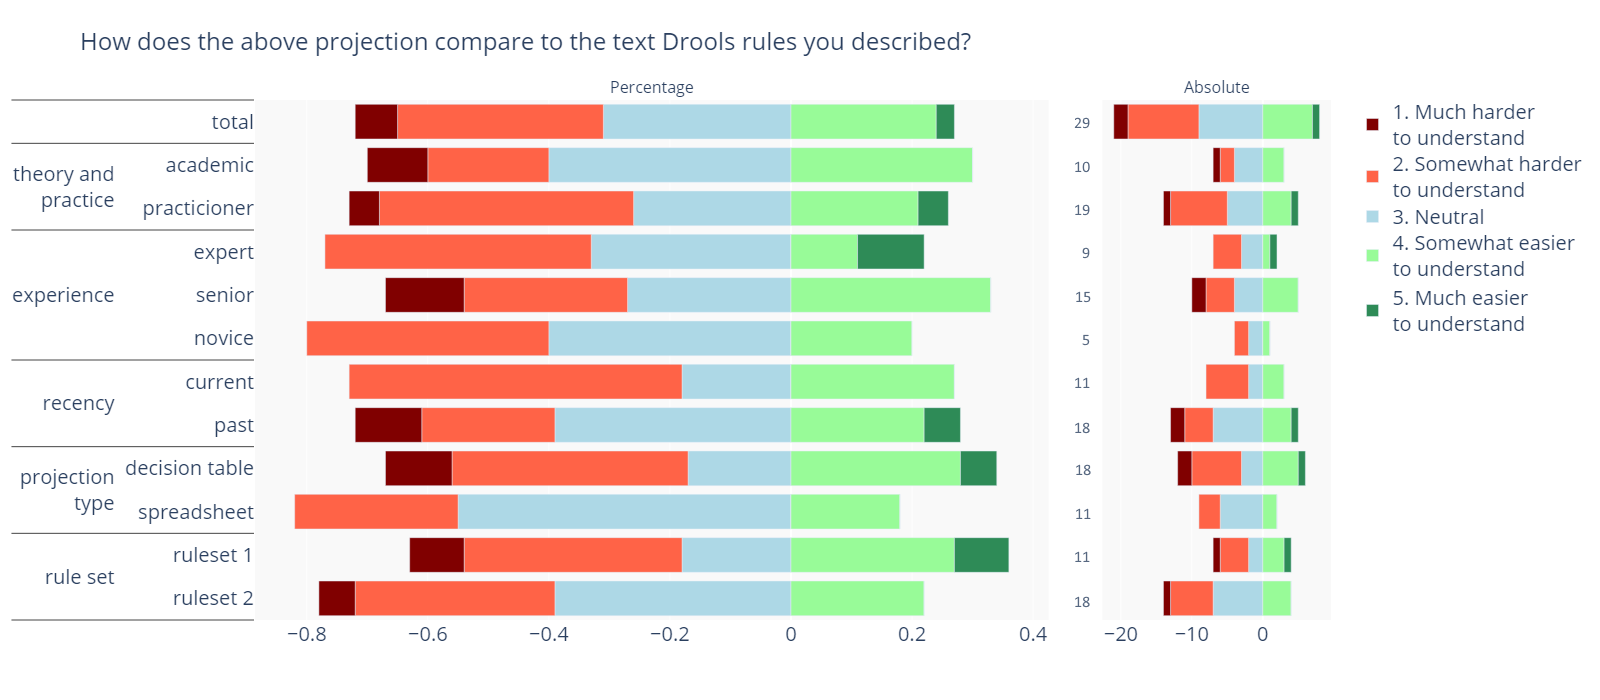
\includegraphics[width=0.95\textwidth]{Sections/images/stackedbar_Q5_2.png}}
    \captionof{figure}{Question 9 - compare projections with text}
    \label{fig:stackedbar_Q5}
    
    \begin{tabular}{ |l ||r |r |r | r|l | } 
        \hline
        Group Comparison                 & Critical U & U-value & z-Score  & p-value & Hypothesis         \\
        \hline
        \hline
        Academic vs Practitioner         & 52         & 85.5    & -0.41295 & 0.6818  & H\textsubscript{0} \\ 
        \hline
        Expert vs Senior                 & 34         & 67.5    & 0.02981  & 0.97606 & H\textsubscript{0} \\ 
        \hline
        Current vs Past                  & 55         & 88      & 0.47194  & 0.63836 & H\textsubscript{0} \\ 
        \hline
        Decision Table vs Spreadsheet    & 55         & 89.5    & -0.40452 & 0.68916 & H\textsubscript{0} \\ 
        \hline
        Ruleset 1 vs Ruleset 2           & 55         & 94.5    & -0.17979 & 0.85716 & H\textsubscript{0} \\ 
        \hline
    \end{tabular}
    \captionof{table}{Mann-Whitney test question 9 - compare projections with text}
    \label{table:mannwhitneyQ5}
\end{minipage} 

This question asked our subjects to compare a tabular projection with the text projection.
There was one participant that chose not to answer this question.

This result, shown in figure \ref{fig:stackedbar_Q5}, was pretty definitive.
The subjects found very much that the textual projections were more understandable than the tabular projections.
The ratio of harder to easier to understand was 3:2, with 12 subjects finding the text projection easier and eight finding the tabular projection easier.
Table \ref{table:mannwhitneyQ5} shows this was independent of any other factors.

\subsubsection{Question 10: Truth Table Validation}
\noindent\begin{minipage}{\linewidth}
    \centering
    \fbox{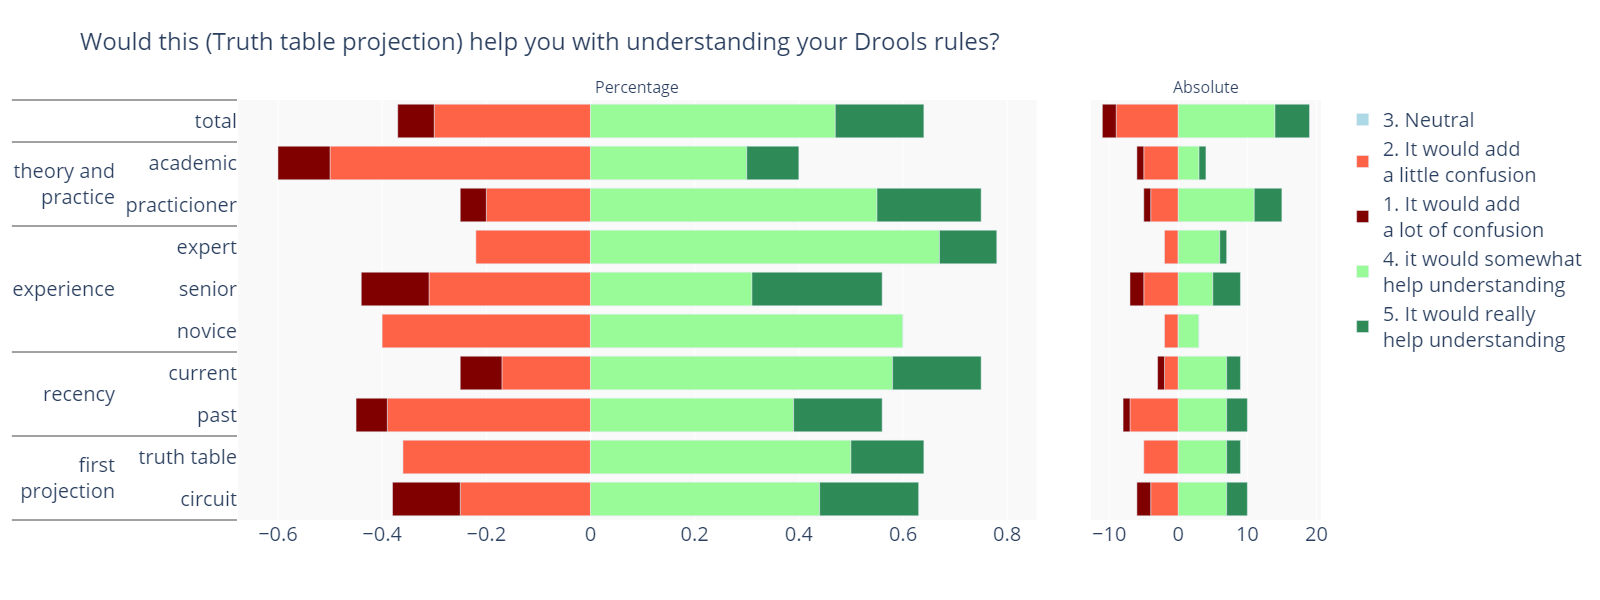
\includegraphics[width=0.95\textwidth]{Sections/images/stackedbar_Q6_2.png}}
    \captionof{figure}{Question 10 - truth table}
    \label{fig:stackedbar_Q6}

    \begin{tabular}{ |l ||r |r |r | r|l | } 
        \hline
        Group Comparison                   & Critical U & U-value & z-Score  & p-value & Hypothesis         \\
        \hline
        \hline
        Academic vs Practitioner           &  55        & 65      & 1.5178   & 0.12852 & H\textsubscript{0} \\ 
        \hline
        Expert vs Senior                   &  37        & 64      & -0.4246  & 0.67448 & H\textsubscript{0} \\ 
        \hline
        Current vs Past                    &  61        & 93      & -0.61383 & 0.54186 & H\textsubscript{0} \\ 
        \hline
        Truth table first vs Circuit first &  64        & 108.5   & -0.12471 & 0.90448 & H\textsubscript{0} \\ 
        \hline
    \end{tabular}
    \captionof{table}{Mann-Whitney test question 10 - truth table}
    \label{table:mannwhitneyQ6}
\end{minipage} 

This question presented the subject with a wireframe of a truth table and asked if it would help them understand rules.

Every subject had a positive or negative view of the projection.
0 of the 30 subjects gave a neutral result.
We found this an improbable result.

There was a net positive view of this projection, with a little less than 2:1 finding it more helpful (19) than confusing (11).

On the first view of the chart in figure \ref{fig:stackedbar_Q6}, it seems that academics have a much more negative view of this projection, and experts have a more positive outlook.
However, when the figures are examined under Mann-Whitney, as seen in table \ref{table:mannwhitneyQ6}, these differences were not statistically significant.

\subsubsection{Question 11: Circuit Diagram Validation}
\noindent\begin{minipage}{\linewidth}
    \centering
    \fbox{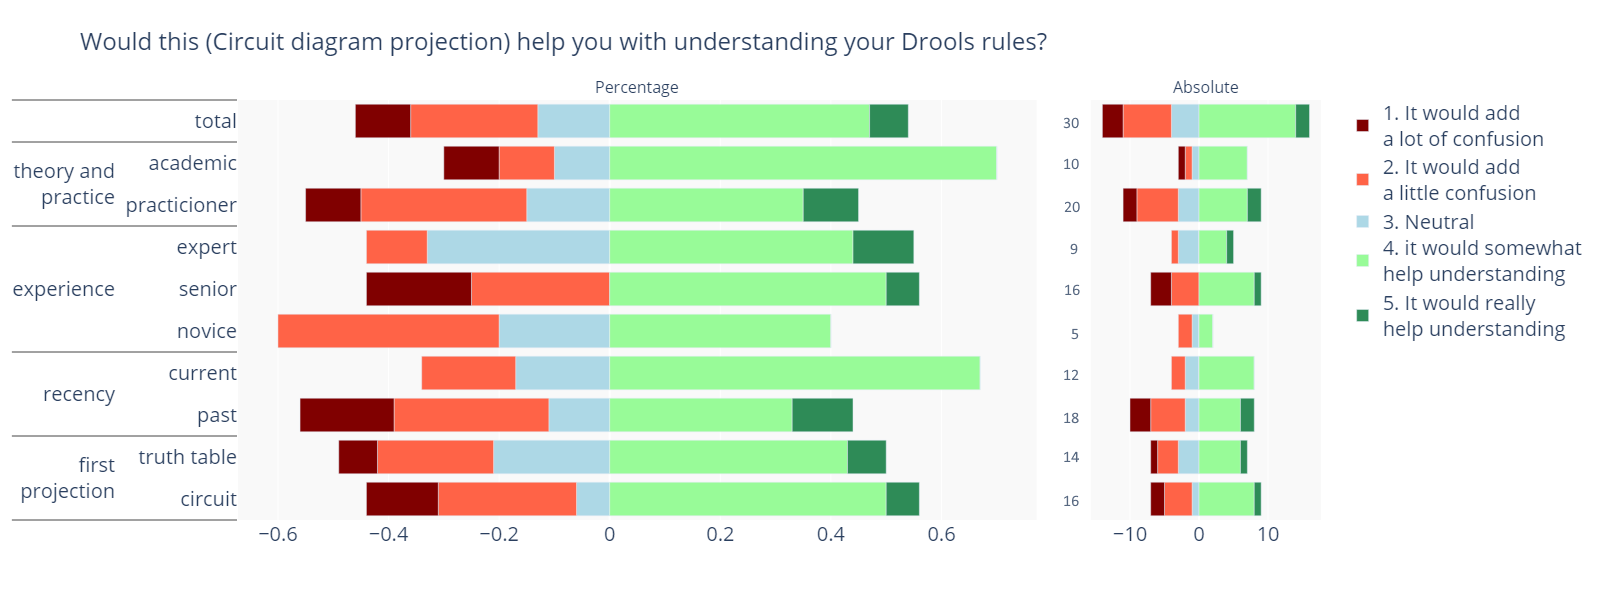
\includegraphics[width=0.95\textwidth]{Sections/images/stackedbar_Q7_2.png}}
    \captionof{figure}{Question 11 - circuit diagram}
    \label{fig:stackedbar_Q7}
    
    \begin{tabular}{ |l ||r |r |r | r|l | } 
        \hline
        Group Comparison                   & Critical U & U-value & z-Score  & p-value & Hypothesis         \\
        \hline
        \hline
        Academic vs Practitioner           & 55         & 83      & -0.7259  & 0.4654  & H\textsubscript{0} \\ 
        \hline
        Expert vs Senior                   & 37         & 58.5    & -0.73598 & 0.4593  & H\textsubscript{0} \\ 
        \hline
        Current vs Past                    & 61         & 83      & -1.03717 & 0.29834 & H\textsubscript{0} \\ 
        \hline
        Truth table first vs Circuit first & 64         & 110     & -0.06236 & 0.95216 & H\textsubscript{0} \\ 
        \hline
    \end{tabular}
    \captionof{table}{Mann-Whitney test question 11 - circuit diagram}
    \label{table:mannwhitneyQ7}
\end{minipage} 

This question presented the subject with a wireframe of a circuit diagram and asked if it would help them with understanding.

The view of the circuit diagram was a net positive, with a ratio of \~3:2 (16 positive, ten negative).

\subsubsection{Question 15: Closing Remarks}

Our last question asks for any last comments.
Sixteen participants decided to add some words.

We ran sentiment analysis on these 16 comments, using the same service and similar code as we used in our SLR research, as described in section \ref{section:dataExtraction}.
Nine were positive, six mixed and one negative.

Figure \ref{fig:Q15_wordcloud} shows another word cloud visualisation.

\begin{figure}[h]
    \centering
    \fbox{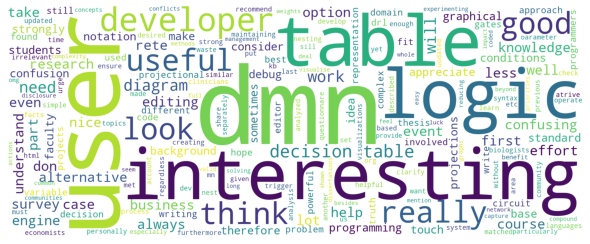
\includegraphics[width=0.95\textwidth]{Sections/images/Q15_wordcloud.png}}
    \caption{Question 15 - responses}
    \label{fig:Q15_wordcloud}
\end{figure}

The word that pops out, DMN, here is indicative of a few comments.
DMN is a tool for working with Drools as a non-developer.
There were some comments that our research should look in this direction.

The feeling was that the projections would give more advantages to non-developers.

There were some hints as to how to improve our projections or other projections to try.
Others suggested that the projections cannot capture some of the complexity of the rules that exist.


\newpage
\section{Discussion - Survey}
\label{section:survey_discussion}

\subsection{Threats to Validity}  

\subsubsection{Construct Validity}
The most prominent issue with this survey is whether it is generalisable to the initial questions it was trying to answer.
The question being ``can projectional editing be used to increase the comprehensibility of large Business rules files?''
There is a solid case that this questionnaire did not ask the right questions to answer this question.
It is difficult to simulate large business rules files in a brief questionnaire.
Comparing the projections to relatively small and non-complex rules collections may not be generalisable to a significant rules collection.

We perhaps had an issue with a mono-operation bias because we only used one tool for measuring - the survey.
We performed many techniques, such as changing orders of questions, measurement, to try and overcome this.
However, all the subjects were still only answering a survey delivered through the same medium - SurveyMonkey.

A possible twist on the response bias may occur from two fronts, where parties may participate in hypothesis guessing and answer questions based on their outcome.
Firstly, two of the respondents were directly known to us, one through work and another through meetings at conferences.
This relationship could have coloured their responses toward a more positive view of our work.
Second, two people who responded were part of the Drools core development team and thus work for JBoss/RedHat.
On top of that, all the people who answered through the Drools consultants mailing list possibly had a direct monetary relationship with RedHat.
This relationship could influence their response towards a more positive view of the status quo.  

\subsubsection{Internal Validity}
Whilst we felt we had tried to overcome the apprehension of the subject being judged when answering questions, the fact that one of our questions asked the subject to describe a Drools rule's meaning could overrule all our previous attempts to assuage that fear.

As with all surveys, the higher the sample size, the greater the chance of validity.
It is difficult to measure the validity of our outcomes due to the relatively small size of our survey.
While 30 respondents are on the low side for using statistical tools to give reasonable responses, statistical validity is also a function of population size.
We requested the size of Drools users from a member of the core Drools development team.  
Unfortunately, that number was not known.
The cross-factor comparisons between the subgroups are of dubious validity as their sample sizes were so small.

\subsubsection{External Validity}
Whilst we feel we reached the right audience of tool users, there was a potential for a geographical selection bias in our population selection technique.
Because a portion of our respondents came from our connections on LinkedIn, and we are from Europe, then there is a particular European bias to our respondents.
Only four of our completed surveys were not from Europe.

There is also a self-selection bias in the sampling. 
As this survey is voluntary, and there is no real personal connection between the subjects and us, then the people who would answer this question are the sort of people who would answer an unsolicited questionnaire.
This bias may affect generalisability to novices, as there was a tendency towards experts in answering the survey.

\subsubsection{Reliability}
Much like our SLR analysis, we also have the credible threat of a single researcher.
All surveys have a subjective nature in their scoring.
Our measurement did not consider cultural differences in question answering between the Dutch and Italians, for example.

\subsubsection{Repeatability vs Reproducibility}
Repeatability is difficult as the survey is about a particular implementation of a particular tool.
However, our survey could be valid with a different underlying tool, and our population sample selection could work for other researchers.

\subsubsection{Method improvement}
We feel our largest problem was smallness.
We would have tried various measures to increase our sample size if we were to try this again.
These would include contacting people directly within LinkedIn, rather than only those whose email addresses or Twitter handles we could harvest.
Also, we would have followed up on the partially completed questionnaires.
Another option would be to select a more extended period for academic papers from which to harvest addresses.

To overcome our mono-operation bias, we could interview people in person.
\newpage

\section{Summary}
In this chapter, we presented a description of the details of the survey we conducted.
Thirty, mostly experience or expert, Drools users responded. 

The goal of this survey was to find if users of Drools would find the projections we used useful.
The outcome seems to be that they seem helpful, but not better than the text they are currently used to.

We tried to control for different groupings that may affect the responses, and in most cases, we found no significant differences in the groups we presented.
There was a significant difference between the projections presented, with the sample, in general, preferring the spreadsheet projection over the decision table. 
